\vspace{1cm}
\fancyhead[C]{\normalsize\textbf{$\qquad$ Teil I: Offene Aufgaben}}
\renewcommand{\labelenumi}{\theenumi.}
\section*{Aufgabe 1 (36 Punkte)}
\vspace{0.4cm}
\subsection*{\aufgabe{a1}{6}}
Für Preise $ p \in [0,3] $ kann der Markt für ein bestimmtes Gut beschrieben werden durch die Angebotsfunktion
\begin{align*}
q_s : \mathbb{R}_+ \to \mathbb{R}, p \mapsto q_s(p)=  4 e^{p-1}
\end{align*}
und die Nachfragefunktion 
\begin{align*}
q_d: \mathbb{R}_+ \to \mathbb{R}, p \mapsto q_d(p) = 70 -15p -1.5p^2.
\end{align*}
Beweisen Sie: Es gibt genau ein Marktgleichgewicht $ (p^\star,q^\star) $ mit Gleichgewichtspreis $ p^\star \in [2,3]$ und Gleichgewichtsmenge $ q^\star \in \mathbb{R}_+ $.\\
\\
\textbf{Lösung:}
\begin{mdframed}
\underline{\textbf{Vorgehensweise:}}
\renewcommand{\labelenumi}{\theenumi.}
\begin{enumerate}
\item Bedingung für Marktgleichgewicht: Angebot = Nachfrage.
\item Zeige, dass ein solches Gleichgewicht in dem gesuchten Intervall vorliegt.
\end{enumerate}
\end{mdframed}
\underline{1. Bedingung für Marktgleichgewicht: Angebot = Nachfrage}\\
Wenn ein Marktgleichgewicht $ (p^\star, q^\star) $ vorliegt, gilt
\begin{align*}
q^\star = q_s(p^\star) = q_d(p^\star)
\ \Leftrightarrow \
q_s(p^\star) - q_d(p^\star) = 0.
\end{align*}
\ \\
\underline{2. Zeige, dass ein eindeutiges Gleichgewicht in dem gesuchten Intervall vorliegt}\\
Nach unserer Vorüberlegung müssen wir die Nullstellen von
\begin{align*}
f(p) := q_s(p) - q_d(p) 
=4 e^{p-1} - 70+15p+1.5p^2
\end{align*}
im Intervall $ [2,3] $ bestimmen.
Ist diese eindeutig, also gibt es nur eine Nullstelle, ist das Marktgleichgewicht eindeutig. Dies wollen wir nun nachweisen.\\
Zuerst verwenden wir den Nullstellensatz von Bolzano, um die Existenz einer solchen Nullstelle zu beweisen:
\begin{align*}
f(2) &= 
4 e^{2-1} - 70 + 15 \cdot 2 + 1.5 \cdot 2^2
=
4 e - 70 + 15 \cdot 2 + 1.5 \cdot 4
= 4 e -34 < 0\\
f(3) &= 
4 e^{3-1} - 70 + 15 \cdot 3 + 1.5 \cdot 3^2
=4 e^2 - 11.5 >0.
\end{align*}
Wegen $ f(2)< 0  $ und $ f(3) > 0  $ muss es wegen der Stetigkeit von $ f $ mindestens ein $ p \in (2,3) $ geben, sodass $ f(p) = 0 $ gilt.\\
Nun fehlt noch die Eindeutigkeit, d.h. es gibt exakt eine Nullstelle in dem Intervall $ [2,3] $. Hierfür betrachten wir die Ableitung:
\begin{align*}
f^\prime(p) = 4 e^{p-1} + 15 +3 p.
\end{align*}
Für diese gilt $ f^\prime(p) > 0  $ für alle $ p \in [2,3] $, womit $ f  $ streng monoton wachsend ist.
Damit nimmt $ f $ in $ [2,3] $ exakt eine Nullstelle an.
Sei $ p^\star  $ diese eindeutige Nullstelle. Dann gilt
\begin{align*}
q^\star = q_s(p^\star)  = q_d(p^\star),
\end{align*}
womit das Marktgleichgewicht eindeutig ist.
\newpage

\subsection*{\aufgabe{a2}{6}}
Für Preise $ p \in [0,3] $ kann der Markt für ein bestimmtes Gut beschrieben werden durch die Angebotsfunktion
\begin{align*}
q_s : \mathbb{R}_+ \to \mathbb{R}, p \mapsto q_s(p) 4 e^{p-1}
\end{align*}
und die Nachfragefunktion 
\begin{align*}
q_d: \mathbb{R}_+ \to \mathbb{R}, p \mapsto q_d(p) = 70 -15p -1.5p^2.
\end{align*}
Der Markt hat genau ein Marktgleichgewicht $ (p^\star,q^\star) $ mit $ p^\star \in [2,3] $.\\
Berechnen Sie $ p^\star  $ näherungsweise mit Hilfe eines Taylorpolynoms 2. Ordnung in $ p_0 = 1 $.
\\
\\
\textbf{Lösung:}
\begin{mdframed}
\underline{\textbf{Vorgehensweise:}}
\renewcommand{\labelenumi}{\theenumi.}
\begin{enumerate}
\item Leite das Taylorpolynom 2. Ordnung in $ p_0 = 1 $ her.
\item Approximiere den Marktgleichgewichtspreis.
\end{enumerate}
\end{mdframed}

\underline{1. Leite das Taylorpolynom 2. Ordnung in $ p_0 = 1 $ her}\\
Wir wissen aus der vorherigen Aufgabe, dass der Marktgleichgewichtspreis $ p^\star $ der eindeutigen Nullstelle in $ [2,3] $ der Funktion
\begin{align*}
f(p) := q_s(p) - q_d(p) 
=4 e^{p-1} - 70+15p+1.5p^2
\end{align*}
entspricht.
Für die Ableitungen gilt
\begin{align*}
f(p)  =4 e^{p-1} - 70+15p+1.5p^2 \ &\Rightarrow \ f(1) = -49.5  \\
f^\prime(p) = 4 e^{p-1}  +15+3p \ &\Rightarrow \ f^\prime(1) = 22\\
f^{\prime \prime}(p) = 4 e^{p-1}  +3
\ &\Rightarrow \
f^{\prime \prime}(1) = 7.
\end{align*}
Damit erhalten wir das 2. Taylorpolynom in $ p_0 = 1  $ durch:
\begin{align*}
P_2(p)
&= 
f(1) + f^\prime(1) (p - 1) + \frac{f^{\prime \prime}(1)}{2} (p-1)^2
=
-49.5 + 22 (p-1) + \frac{7}{2} (p-1)^2\\
&=
-49.5 +22p -22 + \frac{7}{2}(p^2 -2p+1)
=
\frac{7}{2} p^2 + 15 p - 68
\end{align*}
\ \\

\underline{2. Approximiere den Marktgleichgewichtspreis}\\
Um den eindeutigen Marktgleichgewichtspreis zu approximieren, bestimmen wir die Nullstellen von $ P_2 $.
Diese erhalten wir durch
\begin{align*}
P_2(p) = 0
\ \Leftrightarrow \
\frac{7}{2} p^2 + 15 p - 68 = 0
\ \Leftrightarrow \
p = 
\frac{-15 \pm \sqrt{15^2 -4 \frac{7}{2} (-68)}}{2 \frac{7}{2}}
=
\frac{-15 \pm \sqrt{1177}}{7}.
\end{align*}
Wegen $ \sqrt{1177} > 0 $ ist 
\begin{align*}
\frac{-15 - \sqrt{1177}}{7} < 0
\end{align*}
und liegt somit nicht in $ [2,3] $. Des Weiteren gilt
\begin{align*}
\frac{-15 + \sqrt{1177}}{7} \approx 2.7582.
\end{align*} 
Damit ist der approximierte Gleichgewichtspreis durch $ p^\star \approx 2.7582$ gegeben.

\newpage
\subsection*{\aufgabe{b}{10}}
Nina entschliesst sich am Anfang des Jahres, in dem sie ihr Studium beginnt, einen Studienkredit
von CHF $ 100'000 $ aufzunehmen. Sie tut dies trotz des hohen Zinssatzes von $ i = 8 \% $, weil
vertragsgemäss die Zahlung der Zinsen und die Rückzahlung erst im Jahr nach Abschluss ihres
Studiums beginnt.
Dann sollen der Kredit und die Zinsen in $ 10  $ gleichmässigen Raten $ C $, jeweils am Jahresende bezahlt werden.\\
Nina schliesst ihr Studium nach $ 5\frac{1}{2} $ Jahren ab. (\textit{Hinweis: Sie hat damit noch $ 18  $ Monate, bis die erste Rate fällig wird.})
\begin{enumerate}
	\item[(b1)]
	Zeichnen Sie die beschriebenen Zahlungsströme und Ereignisse an einem Zeitstrahl an.
	\item[(b2)] 
	Wie hoch sind Nina's Schulden zu Beginn des Jahres in dem die Rückzahlung beginnt?
	\item[(b3)] 
	Bestimmen Sie die Höhe der vereinbarten Raten $ C $.
\end{enumerate}
Nachdem sie schon $ 5 $ Raten abbezahlt hat, macht Nina eine Erbschaft von CHF $ 100'000 $.
Sie beschliesst, statt der $ 6. $ Rate den ganzen Restbetrag zurückzuzahlen.
\begin{enumerate}
	\item[(b4)] 
	Ergänzen Sie die Info am Zeitstrahl.
	\item[(b5)] 
	Reichen die CHF $ 100'000 $, um die Schulden vollkommen zurückzuzahlen?\\
	Wenn ja: Wie viel bleibt Nina von ihrer Erbschaft?\\
	Wenn nein: Welchen zusätzlichen Betrag muss Nina zur Tilgung ihrer Schulden aufbringen?
\end{enumerate}
\ \\
%\textbf{Lösung:}
%\begin{mdframed}
%\underline{\textbf{Vorgehensweise (b1) - (b3):}}
%\begin{enumerate}
%\item (b1) Zeichne die Zahlungsströme und Ereignisse in einen Zeitstrahl ein.
%\item (b2) Überlege dir, wie hoch die Schuldenlast zu Beginn der Rückzahlung ist.
%\item (b3) Rufe dir eine passende Formel für die Rate in Erinnerung und berechne diese.
%\item 
%(b4) Zeichne das aktualisierte Schaubild.
%\item 
%(b5) Überlege dir, ob die Erbschaft reicht um den Restbetrag zurückzuzahlen.
%\end{enumerate}
%\end{mdframed}

\underline{(b1) Zeichne die Zahlungsströme und Ereignisse in einen Zeitstrahl ein:}\\
Die Zahlungsströme und Ereignisse lassen sich folgendermaßen
grafisch darstellen:
\begin{center}
	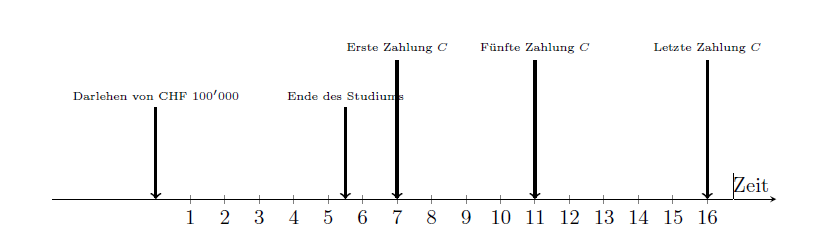
\includegraphics{pictures/zeitstrahl_1}
\end{center}
\newpage
\underline{(b2) Überlege dir, wie hoch die Schuldenlast zu Beginn der Rückzahlung ist:}\\
Da Nina erst im Jahr nach Abschluss ihres Studium mit den Rückzahlungen beginnt und die Raten $ C $ zum Jahresende gezahlt werden, entspricht der Kredit am Anfang von Jahr $ 7 $ einer Verzinsung von $ 6  $ Jahren.
Demnach gilt
\begin{align*}
A_6 = A_0 (1 + i)^6
= 100'000 (1+0.08)^6 \approx 158'687.45 (CHF)
\end{align*}
nach $ 6 $ Jahren.\\
\\
\underline{(b3) Benutze die Formel für eine nachschüssige Rente, um $ C $ zu bestimmen:}\\
Beginnend im $ 6. $ Jahr haben wir zehn jährliche Zahlungen $ C $ zum Ende des Jahres.
Dies entspricht einer nachschüssigen Rente mit dem Anfangswert $ P  = A_6 $, $ n = 10  $ und $ i = 8 \% $.
Damit erhalten wir 
\begin{align*}
C = \frac{i}{(1+i)^n-1}(1+i)^n P
=\frac{i P}{1 - (1+i)^{-n}}
=
\frac{0.08 \cdot 158'687.45}{1-(1+0.08)^{-10}}
\approx 
23'649.10 (CHF)
\end{align*}
als jährliche Rate für Nina.\\
\\
\underline{(b4) Zeichne das aktualisierte Schaubild:}\\
Das aktualisierte Schaubild ist gegeben durch:
\begin{center}
	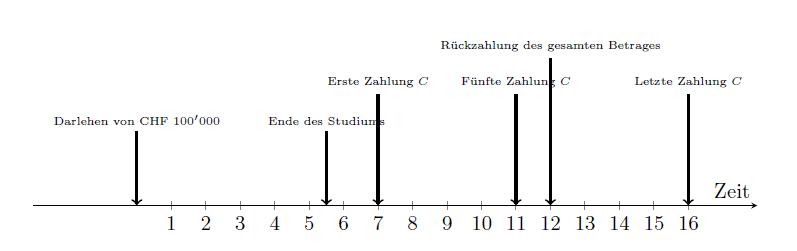
\includegraphics{pictures/zeitstrahl_2}
\end{center}
\ \\
\underline{(b5) Bestimme den noch offenen Restbetrag:}\\
Angenommen wir hätten die Schuld bis zu Beginn des $ 12. $ Jahres nicht getilgt.
Dann haben wir eine offene Schuld von
\begin{align*}
A_{12} = A_0 (1+i)^{12} = 100'000(1+0.08)^{12}
\end{align*}
zu Beginn des 12. Jahres, falls keine jährlichen Zahlungen geflossen sind.
Die jährlichen Zahlungen über 5 Jahre setzen sich zusammen aus
\begin{align*}
C \sum \limits_{k=1}^5 (1+ 0.08)^k
= C \cdot 1.08+ ... + C\cdot (1.08)^5.
\end{align*}
Dies liefert uns die Rückzahlung über die Jahre der Rückzahlung verzinst.
Damit erhalten wir die offene Schuld für Nina mithilfe der geometrischen Summe:
\begin{align*}
A_{12} - C \sum \limits_{k=1}^5 (1+ 0.08)^k
=
100'000(1+ 0.08)^{12}- 23'649.1 \cdot 1.08 \frac{1.08^5 -1}{0.08}
\approx 101'977.95 (CHF).
\end{align*}
Damit kann die offene Schuld nicht durch die Erbschaft beglichen werden.
Sie muss noch $ 1977.95 (CHF) $ zusätzlich tilgen. \\
\\
\textit{Hinweis:} Diese Aufgabe zeigt sehr, wie sich der Zinseszinseffekt auswirkt.
Überlegen sie sich immer sehr gut, ob und zu welchem Zweck sie sich verschulden.
\newpage
\subsection*{\aufgabe{c}{5}}
Im Jahre 1955 entwickelte Morris Swadesh (1909-1967) eine (umstrittene) Methode, die sog.
Glottochronologie, um den Zeitpunkt zu bestimmen, an dem zwei verwandte Sprachen (z. B.
Latein und Sanskrit) sich verzweigten. Swadesh ging von der Hypothese aus, dass die sprachlichen
Atome - d.h. die Wörter - zerfallen wie radioaktive Atome. Laut Voraussetzung soll der
grundlegende Urwortschatz der Sprachen mit einer Halbwertszeit von etwa 2000 Jahren aussterben.
Kennt man die Menge des noch gemeinsamen Urwortschatzes zweier Sprachen und geht
davon aus, dass sich diese Menge alle 2000 Jahre halbiert, kann man berechnen, wann sich
die Sprachen verzweigt haben. A. Raun und E. Kangsmaa-Minn führten unabhänging voneinander,
d.h. jeweils mit einer eigenen Methode, den Vergleich des Finnischen und Ungarischen
durch. Während Raun herausfand, dass der Anteil der identischen Elemente in beiden Sprachen
$21 \% $ beträgt, berechnete Kangsmaa-Minn einen Anteil von $ 27 \% $.\\
Innerhalb welches Zeitraums haben sich die beiden Sprachen nach der Theorie der Glottochronolgie
und aufgrund dieser Zahlen voneinander getrennt?\\
\\
\textit{Bemerkung}:\\
Berechnen Sie also, vor wie vielen Jahren sich das Finnische und das Ungarische gemäss a)
der Berechnung von A. Raun und b) der Berechnung von E. Kangsmaa-Minn getrennt haben.
Geben Sie das finale Ergebnis als Zeitintervall an.\\
\\
\textbf{Lösung:}
\begin{mdframed}
\underline{\textbf{Vorgehensweise:}}
\begin{enumerate}
\item Leite eine Formel für die Prozentzahl identischer Elemente in der Finnische und Ungarischen Sprache her.
\item Wende diese Formel an, um das Zeitintervall herzuleiten.
\end{enumerate}
\end{mdframed}

\underline{1. Leite eine Formel für die Prozentzahl identischer Elemente in der Finnische und Ungarischen Sprache her}\\
Wir betrachten $ G(t) $ formal als die Prozentzahl identischer Elemente in der Finnischen und Ungarischen Sprache $ t $ Jahre nach deren Trennung. Dann gilt 
\begin{align*}
G(0) = 100 %,
\end{align*}
da zum Zeitpunkt der Trennung die Sprachen identisch sind.
Des Weiteren gilt
\begin{align*}
\frac{G(t+2000)}{G(t)} = \frac{1}{2}.
\end{align*}
Insgesamt erhalten wir als explizite Formel
\begin{align*}
G(t) = 100 \% \left(\frac{1}{2}\right)^{\frac{t}{2000}}.
\end{align*}
\newpage
\underline{2. Wende diese Formel an, um das Zeitintervall herzuleiten}\\
Die beiden Wissenschaftler liefern uns eine identische Übereinstimmung der Sprachen von $ 21\% $ bis $ 27 \% $.
Demnach gilt
\begin{align*}
21 \% \leq 100 \% \left(\frac{1}{2}\right)^{\frac{t}{2000}} \leq 27 \%
\ 
&\Leftrightarrow
\
0.21 \leq 1 \left(\frac{1}{2}\right)^{\frac{t}{2000}} \leq 0.27\\
\ &\Leftrightarrow \
\ln(0.21) \leq \ln\left( \left(\frac{1}{2}\right)^{\frac{t}{2000}}  \right) \leq \ln(0.27)\\
\ &\Leftrightarrow \
\ln(0.21) \leq \frac{t}{2000} \ln \left(\frac{1}{2}\right) \leq \ln(0.27)\\
\ &\Leftrightarrow \
\ln(0.21) 2000 \leq t \underbrace{\ln \left(\frac{1}{2}\right)}_{< 0} \leq \ln(0.27) 2000\\
\ &\Leftrightarrow \
\frac{\ln(0.27)}{\ln(0.5)} 2000 \leq t  \leq \frac{\ln(0.21)}{\ln(0.5)} 2000 \\
\ &\Leftrightarrow \
3778 \leq t  \leq 4503.
\end{align*}
Also liegt der Zeitraum in dem sich die Finnische und Ungarische Sprache getrennt haben zwischen $ 3778 $ und $ 4503 $ Jahren.
\newpage

\subsection*{\aufgabe{d}{9}}
Ein Student hat ein gegenwärtiges Einkommen von CHF $ 3'000 $ und erwartet in einem Jahr ein zukünftiges Einkommen von CHF $ 7'000 $. Er plant einen gegenwärtigen Konsum $ c_1 $ und im
folgenden Jahr einen Konsum $ c_2 $ mit der Absicht die Nutzenfunktion $ u = \ln(c_1) + \frac{1}{1.2}
\ln(c_2) $ zu maximieren.\\
Wenn er jetzt Geld leiht, weil $ c_1 > 3'000 $ CHF ist, dann wird der zukünftige Konsum $ c_2 $ nach
Rückzahlung des Kreditbetrages und der Zinsen berechnet. Spart er entsprechend Geld, i. e.
$ c_1 < 3'000 $ CHF, dann kann er $ c_2 $ um den gesparten Betrag und dessen Zinsen erhöhen. Der (optimistische)
Zinssatz für Leihen und Sparen beträgt $ i = 8\% $.
\begin{enumerate}
	\item[(d1)] Bestimmen Sie den Zusammenhang zwischen $ c_1 $ und $ c_2 $.
	\item[(d2)] Bestimmen Sie den Nutzen des Studenten in Abhängigkeit von $ c_1 $.
	\item[(d3)] Für welche Wahl von $ c_1 $ ist der Nutzen des Studenten maximal?\\
	Wie viel muss er sich allenfalls leihen? 
\end{enumerate}
\ \\
\\
\textbf{Lösung:}
\begin{mdframed}
	\underline{\textbf{Vorgehensweise:}}
	\begin{enumerate}
		\item (d1) Überlege dir, was für die Barwerte von Konsum und Einkommen gelten muss.
		\item 
		(d2) 
		Verwende die letzte Teilaufgabe.
		\item 
		(d3) Bestimme das Maximum der Nutzenfunktion.
	\end{enumerate}
\end{mdframed}

\underline{1. (d1) Überlege dir, was für die Barwerte von Konsum und Einkommen gelten muss}\\
Die Barwerte von Konsum und Einkommen müssen identisch sein.\\
\\
Der Barwert des Konsums ist: 
\begin{align*}
c_1 + \frac{c_2}{(1+0.8)}= c_1 + \frac{c_2}{1.08}.
\end{align*}
Der des Einkommens ist:
\begin{align*}
3'000 + \frac{7'000}{(1+0.08)}
=
3'000 + \frac{7'000}{1.08}.
\end{align*}
Damit muss 
\begin{align*}
c_1 + \frac{c_2}{1.08}
=
3'000 + \frac{7'000}{1.08}
&\Leftrightarrow
1.08 c_1 + c_2 = 3'000 \cdot 1.08 + 7'000\\
&\Leftrightarrow
c_2 = 3'000 \cdot 1.08 + 7'000 - 1.08 c_1 \\
&\quad \quad  \ = 10'240 - 1.08 c_1
\end{align*}
gelten.\\

\newpage
\underline{(d2) Verwende die letzte Teilaufgabe}\\
Aus der Teilaufgabe (d1) wissen wir, dass
\begin{align*}
c_2 = 10'240 -1.08 c_1
\end{align*}
gilt. Eingesetzt in unsere Nutzenfunktion ergibt sich
\begin{align*}
u(c_1,c_2) 
=
\ln(c_1) + \frac{1}{1.2} \ln(c_2)
=
\ln(c_1) + \frac{1}{1.2} \ln(10'240 -1.08 c_1)
=: v(c_1).
\end{align*}
Somit hängt die Nutzenfunktion nur noch von $ c_1 $ ab.\\
\\
\underline{3. (d3) Bestimme das Maximum der Nutzenfunktion}\\
Zunächst bestimmen wir die Ableitung von $ v $:
\begin{align*}
v^\prime( c_1 ) 
=
\frac{1}{c_1}- \frac{1.08}{1.2 }\cdot \frac{1}{10'240 - 1.08 c_1}.
\end{align*}
Für das Maximum muss
\begin{align*}
v^\prime(c_1) =  \frac{1}{c_1}- \frac{1.08}{1.2 }\cdot \frac{1}{10'240 - 1.08 c_1} = 0
&\Leftrightarrow
\frac{1}{c_1} =  \frac{1.08}{1.2 }\cdot \frac{1}{10'240 - 1.08 c_1}\\
&\Leftrightarrow
c_1 = \frac{1.2}{1.08}(10'240 - 1.08 c_1)\\
&\Leftrightarrow
2.2 c_1 = \frac{1.2 \cdot 10'240}{1.08}\\
&\Leftrightarrow
c^\star_1 = \frac{1.2 \cdot 10'240}{1.08 \cdot 2.2} \approx 5'171.70 (CHF)
\end{align*}
gelten. Für die zweite Ableitung gilt mit der Kettenregel:
\begin{align*}
v^{\prime \prime}(c_1)
=
- \frac{1}{c_1^2} - \frac{1.08^2}{1.2} \frac{1}{(10'240 - 1.08 c_1)^2} < 0
\end{align*}
Damit liegt an $ c_1^\star  $ ein globales Maximum vor.
Also gilt auch 
\begin{align*}
c_2^\star = 10'240 - 1.08 c_1^\star
\approx
4'654.55 (CHF).
\end{align*}
Im ersten Jahr leiht er sich 
\begin{align*}
c_1^\star - 3'000 \approx 2'171.70 (CHF)
\end{align*}
und im zweiten Jahr ist der Konsum $ c_2^\star $ geringer als sein Einkommen.
Jedoch muss er im zweiten Jahr eine Schuld von $ 2'345.45 $ CHF
tilgen.
\newpage